\documentclass[xcolor=dvipsnames]{beamer}
\usepackage[slovak]{babel}
\usepackage{graphicx}
\usepackage[T1]{fontenc}
\usepackage[utf8]{inputenc}
\usepackage{lmodern}
\usepackage{hyperref}
\usepackage{verbatim}
%%\usepackage[slovak, ruled, vlined]{algorithm2e}
%%\newcommand\mycommfont[1]{\footnotesize\ttfamily\textcolor{blue}{#1}}
%%\SetCommentSty{mycommfont}
%%\SetKwFor{For}{for (}{) $\lbrace$}{$\rbrace$}
\usepackage[slovak, linesnumbered,ruled,vlined]{algorithm2e}
\usepackage[dvipsnames]{xcolor}
%------------------------------------------------------
\usetheme{Madrid}
\usecolortheme[named=BlueViolet]{structure}
\setbeamertemplate{itemize items}[square]
\setbeamertemplate{enumerate items}[square]
\setbeamertemplate{sections/subsections in toc}[square]
%------------------------------------------------------
\title[Polia]{{\Huge Polia}}
\subtitle{v~jazyku C}
\institute[]{Vysoké učení technické v~Brně}
\author[Dátové štruktúry ]{Mervart Jaroslav }
\date{2. Mája 2024}
%------------------------------------------------------
\begin{document}
{
\setbeamertemplate{footline}{}
\begin{frame}[noframenumbering]
    \maketitle
\end{frame}
}
%------------------------------------------------------
\section{Úvod}
\begin{frame}{Obsah}
    \tableofcontents[sectionstyle=show]
\end{frame}
%------------------------------------------------------
\begin{frame}{Význam polí }
    \begin{block}{\footnotesize{starofrancúzsky -- arraier (usporiadať)}}
\begin{quote}
    \uv{Pole v~jazyku C je jednou z~najpoužívanejších dátových štruktúr v~programovaní v~jazyku C.} \footnotemark 
\end{quote}
\end{block}
    \begin{itemize}
        \item Výhody
        \begin{itemize}
            \item jednoduchosť
            \item reprezentácia matíc
            \item ukladanie väčšieho počtu prvkov rovnakého typu
        \end{itemize}
        \item Nevýhody
        \begin{itemize}
            \item pevná veľkosť pri vytvorení
            \begin{itemize}
                \item pri staticky alokovaných nemeniteľná
                \item viď sekciu \nameref{dyn_alloc}
            \end{itemize}
            \item rýchlosť (oproti iným dátovým štruktúram)
        \end{itemize}
    \end{itemize}
\footnotetext[1]{\href{https://www.w3schools.com/c/c_arrays.php}{www.w3schools.com}}
\end{frame}
%------------------------------------------------------
\section{Deklarácia a inicializácia}
\begin{frame}{Deklarácia a inicializácia polí}
    \textbf{Deklarácia:} \texttt{int my\_Arr[size]}
    \begin{block}{príklad\:1}
        \texttt{int my\_Arr[5]; // pole s~5 celočíselnými prvkami}
    \end{block}
    
    \textbf{Inicializácia:} \texttt{int my\_Arr[] = \{ x, y, z, \ldots \}}
    \begin{block}{príklad\:2}
        \texttt{int my\_Arr[] = \{1, 2, 3, 4, 5\}; // Inicializuje pole s~danými hodnotami}
    \end{block}
    \begin{alertblock}{Indexácia}
        \centering {Polia indexujeme od 0!}
    \end{alertblock}
\end{frame}
%------------------------------------------------------
\section{Operácie}
\begin{frame}{Operácie s~poliami}

    \textbf{Pristupovanie} k~položke $\longmapsto$ \texttt{my\_Arr [index];}.
    \begin{block}{príklad\:3}
        \texttt{int my\_Arr[] = \{1, 2, 3, 4, 5\} ;\\
        \texttt{int x = my\_Arr[4] ; // \textbf{x = 5}}  
    }
    \end{block}
    \begin{alertblock}{Skúška pozornosti}
        Akú hodnotu by sme v~predošlom príklade dostali z~indexu 5?
    \end{alertblock}
    \textbf{Zmena hodnoty} položky $\longmapsto$ \texttt{my\_Arr[i] = nová\_hodnota;}.
    \begin{block}{príklad\:4}
        \texttt{int my\_Arr[] = \{1, 2, 3, 4, 5\} ;\\
        \texttt{my\_Arr[4] = 20 ; // \texttt{my\_Arr[] = \{1, 2, 3, 4, {\color{red}20}\}}}  
    }
    \end{block}
\end{frame}
%------------------------------------------------------
\section{Viacrozmerné polia}
\begin{frame}{Viacrozmerné polia}
\begin{columns}
\column{0.5\textwidth}
    \begin{itemize}
    \item \textbf{Jednorozmerné pole (1D pole)}:
        \begin{itemize}
            \item napr. \texttt{pole[0]}, \texttt{pole[1]}.
        \end{itemize}
    \item \textbf{Dvojrozmerné pole (2D pole)}:
        \begin{itemize}
            \item Dve dimenzie (riadky a stĺpce).
            \item Deklarácia: \texttt{int a[5][10];}
            \item Prístup k~prvkom: \texttt{a[0][3] = 10;}.
        \end{itemize}
    \item \textbf{Trojrozmerné pole (3D pole)}:
        \begin{itemize}
            \item Tri dimenzie (napr. x, y, z).
            \item reprezentácia trojrozmerných objektov
        \end{itemize}
\end{itemize}
\column{0.5\textwidth}
\begin{figure}
    \centering
    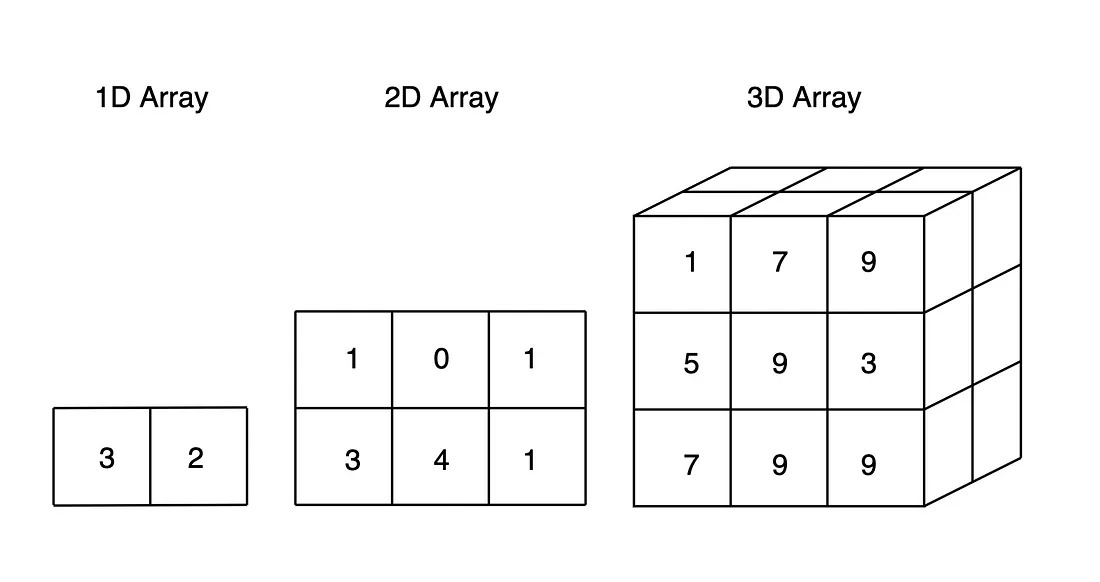
\includegraphics[width=1\linewidth]{latexprez2.jpg}
    \caption{Ukážka priestorov polí \footnotemark}
    \label{fig:1_2_3D_arr_example}
\end{figure}
\end{columns}
\footnotetext[2]{Obrázok prevzatý z~\href{https://towardsdatascience.com/numpy-array-cookbook-generating-and-manipulating-arrays-in-python-2195c3988b09}{www.towardsdatascience.com}}
\end{frame}


\begin{frame}{Viacrozmerné polia -- pokračovanie}
\begin{itemize}
        \item \textbf{Štvorrozmerné pole (4D pole)}:
        \begin{itemize}
            \item Má štyri dimenzie (napr. čas, x, y, z).
            \item Používa sa v~matematike, fyzike alebo pri spracovaní obrazu.
        \end{itemize}
    \end{itemize}
    \begin{figure}
        \centering
        
\includegraphics[width=0.5\linewidth]{latexprez.jpg}
        \caption{Pre pochopenie (nielen) 4D polí -- pole polí.\footnote{Obrázok prevzatý z~\href{https://www.ubeeco.com.au/news/2017/02/12/custom-made-boxes-avoid-set-up-charges/}{www.ubeeco.com.au}}}
        \label{fig:4D_array_example}
    \end{figure}
\end{frame}
%------------------------------------------------------
\section{Dynamická alokácia} \label{dyn_alloc}
\begin{frame}{Dynamická alokácia polí}

\begin{itemize}
    \item funkcia \texttt{malloc()}:
    \begin{itemize}
        \item dynamická alokáciu jedného bloku pamäte s~určitou veľkosťou. 
        \item vracia ukazovateľ typu void (pretypovanie je možné)
        \item \footnotesize\texttt{\color{blue}{ptr = (typ\_pretypovania*) malloc(velkosť\_v\_bytoch)}}
        \item Príklad: \footnotesize\texttt{\color{red}{ptr = (int*)malloc(size * sizeof(int))}}
    \end{itemize}
    \item funkcia \texttt{calloc()}:
    \begin{itemize}
        \item každý blok inicializovaný na hodnotu 0
        \item \footnotesize\texttt{\color{blue}{ptr = (typ\_pretypovania*) calloc(pocet, velkosť\_prvku)}}
        \item Príklad: \footnotesize\texttt{\color{red}{ptr = (int*) calloc(5, sizeof(float))}}
    \end{itemize}
    \item funkcia \texttt{realloc()}:
    \begin{itemize}
        \item zmena veľkosti existujúceho dynamického poľa (zväčšenie alebo zmenšenie)
        \item \footnotesize\texttt{\color{blue}{ptr = realloc(ptr, nová\_veľkosť\_v\_bytoch)}}
        \item Príklad: \footnotesize\texttt{\color{red}{ptr = realloc(ptr, 6);}}
    \end{itemize}
\end{itemize}
\footnotetext[4]{Prevzaté a upravené z~\href{https://www.geeksforgeeks.org/dynamic-array-in-c/}{www.geeksforgeeks.org}}
\end{frame}
%------------------------------------------------------
\section{Zhrnutie}
\begin{frame}{Zhrnutie}
    \begin{itemize}
        \item Polia obsahujú rovnaký typ prvkov, indexovaných od 0.
        \item Vieme pristupovať k~jednotlivým položkám a meniť ich.
        \item Môžeme vytvárať viacrozmerné polia (s~rozumom).
        \item Funkcie \texttt{malloc()}, \texttt{calloc()} a \texttt{realloc()} slúžia na dynamickú alokáciu (nielen) polí a ich správu.
    \end{itemize}
\end{frame}
%------------------------------------------------------
\end{document}
